% This is a sample document using the University of Minnesota, Morris, Computer Science
% Senior Seminar modification of the ACM sig-alternate style. Much of this content is taken
% directly from the ACM sample document illustrating the use of the sig-alternate class. Certain
% parts that we never use have been removed to simplify the example, and a few additional
% components have been added.

% See https://github.com/UMM-CSci/Senior_seminar_templates for more info and to make
% suggestions and corrections.

\documentclass{sig-alternate}
\usepackage{color}
\usepackage[colorinlistoftodos]{todonotes}

\newcommand{\comment}[1]{}
\definecolor{Coquelicot}{RGB}{255, 56, 0}
\newcommand{\pscomment}[1]{\textcolor{Coquelicot}{\comment{Paul: {#1}}}}

%%%%% Uncomment the following line and comment out the previous one
%%%%% to remove all comments
%%%%% NOTE: comments still occupy a line even if invisible;
%%%%% Don't write them as a separate paragraph
%\newcommand{\mycomment}[1]{}

\begin{document}

% --- Author Metadata here ---
%%% REMEMBER TO CHANGE THE SEMESTER AND YEAR
\conferenceinfo{UMM CSci Senior Seminar Conference, December 2013}{Morris, MN}

\title{Usability of Error Messages for Introductory Students}

\numberofauthors{1}

\author{
% The command \alignauthor (no curly braces needed) should
% precede each author name, affiliation/snail-mail address and
% e-mail address. Additionally, tag each line of
% affiliation/address with \affaddr, and tag the
% e-mail address with \email.
\alignauthor
Paul A. Schliep\\
	\affaddr{Division of Science and Mathematics}\\
	\affaddr{University of Minnesota, Morris}\\
	\affaddr{Morris, Minnesota, USA 56267}\\
	\email{schli202@morris.umn.edu}
}

\maketitle
\begin{abstract}
Error messages are an important tool for programmers to help find and fix errors in their code.
When an error message is unhelpful it can be difficult to find and fix the mistakes.
Error messages are especially critical for introductory programmers in understanding problems with their code.
Not all error messages are beneficial for helping novice programmers, however.
This paper discusses the general usability of error messages for introductory programmers and the importance these messages have on learning programming.
After that, we discuss the analyses of DrRacket and C++ compiler error messages.
We then discuss a set of recommendations on improving error messages in development environments and a error enhancement program meant to help improve the experience a novice programmer with error messages, and their effectiveness.

% The current paper format *only* allows inline comments using the todo
% macro. That's kind of a bummer, and it would be neat if someone figured
% out how to change the acmconf style to allow this. I suspect it isn't *hard*
% but there are quite a few details that have to be sorted out in synchrony.
\end{abstract}

\keywords{Novice programmers, usability, error messages, usability studies, compiler errors, syntax errors}


\section{Introduction}\label{sec:intro}
One of the most important foundations of computer programming is the communication between the system and the user, specifically in the error messages produced by the system.
These error messages are especially important for introductory-level computer science students to help them resolve issues in their program because the error messages are the primary source for understanding what is wrong.
According to Marceau et al, ``[students] lack the experience to decipher complicated or poorly-constructed feedback'' ~\cite{Marceau:2011:MEE:1953163.1953308}.
The first rule of good message design is to be sure that the error does not add confusion ~\cite{Isa:1983:MOE:800045.801583}.
Difficulties in understanding error messages often lead to frustration because the error message was either too complicated to understand or led them down the wrong path~\cite{Marceau:2011:MYL:2048237.2048241}, which can sometimes introduce new errors ~\cite{Denny:2014:ESE:2591708.2591748}. 

Several studies have been conducted on modern programming languages' error messages to study the effectiveness in helping novice programmers debug their program and help learn the concepts and programming languages.
The results have shown that students struggle with compiler and syntax error messages ~\cite{Denny:2014:ESE:2591708.2591748,Traver:2010} (which we will discuss in detail in Section 3) and the general vocabulary of the error messages along with IDE-specific features such as source highlighting can be bothersome for introductory computer science students ~\cite{Marceau:2011:MYL:2048237.2048241}. 

Several tools and heuristics are being developed to help address issues in error message usability and its development.
The goals of these methodologies are to help introductory programmers learn the language and concepts easier.
The goal of this paper is to discuss the analyses of error message design and its usability for introductory students in a class setting (meaning students' interactions with programming in a lab setting and at home), and how these developed methodologies help improve the user experience with error messages. 

This paper is divided into five sections.
In Section 2 we discuss usability studies, define compiler, syntax, and runtime error messages, and discuss imperative and functional programming.
In Section 3 we will focus on  analyses of the usability of exception messages and compiler messages for introductory students and how those analyses were performed.
In Section 4 we discuss the results of those analyses.
In Section 5 we introduce three methodologies developed to help improve the error message usability.
The first we will cover is Traver's heuristics for compiler message design ~\cite{Traver:2010}.
Then, we will examine Marceau et al. recommendations for error message design ~\cite{Marceau:2011:MYL:2048237.2048241}.
Lastly, we will explore Denny et al. syntax error enhancement tool ~\cite{Denny:2014:ESE:2591708.2591748}.


\section{Background}\label{sec:background}
In order to discuss the analyses of error messages, we need to understand several concepts related to error types and usability.
These concepts include compiler errors, syntax errors, runtime errors, usability studies, and Human Computer Interaction.
We will also cover dynamically and statically typed languages and their differences.
We will then be discussing the programming languages and tools used in the analysis of the error messages.
They include Racket, C++, and Java programming languages and an overview of Integrated Development Environments (IDEs), and DrRacket in particular. 


\subsection{Human-computer interaction and methods of usability analysis}\label{subsec:hci}

The study of Human-Computer Interaction, or HCI, is focused on how computer technology is used, specifically on the interfaces between the user and the programs of the computer.
As Traver notes, ``HCI is a discipline that aims to provide user interfaces that make working with a computer a more productive, effective, and enjoyable task''~\cite{Traver:2010}.
Much of the research presented in this paper is from an HCI point of view, rather than a more technical approach.
Thus, the areas we are looking at in error message design is the language used in the message, accuracy and precision of the messages, as well as interface elements such as text highlighting.

In order to analyze these messages from an HCI perspective and attain qualitative and quantitative information about their usability, a usability test or case study may be performed.
A usability test is a technique often used in HCI studies to evaluate a program or product by testing it on users.
A case study is a research method that closely studies a group of participants, in the case of this paper, introductory students in a classroom, and collects data about participants by observations and interviews.
Many of the studies performed on error messages analyzed in this paper are using a case study and usability test design. 

\subsection{Compiler and Runtime errors}\label{subsec:error types}

In this paper, we discuss the general usability of error message design, but in order to do so, we will need to define compiler and runtime errors.
Note that when defining these error types, I will be talking about compiled, statically typed languages, which we define at the end of this subsection.
A compiler is a program that converts source code written in a programming language into a language that a computer's processor can read so that instructions can be executed.
A compilation error refers to a state when a compiler fails to compile a piece of  program source code.
A program will not run if there is a compiler error because the compiler will not be able to create executable code to run if there are errors the compiler finds. 
Then, we examine syntax errors, which is a type of compiler error that occurs when the code does not conform to the syntactical order expected by the parser.
Often, these errors occur from variables that are not defined or missing/extra punctuation.
The parser, is a program (usually part of a compiler) that receives input as program instructions and builds it into a structural representation of the input while checking for correct syntax of the input.
As Kummerfield and Kay note ~\cite{Kummerfeld:2003:NBF:858403.858416}, ``The usability of compiler errors are important because syntax error correction is the first step in the debugging process. It is not possible to continue program development until the code compiles. This means it is a crucial part of the error correction process.''
Below is an example of a compiler error. Here, the programmer is defining \texttt{seven} to be \texttt{2+5}, but forgot to close the parenthesis. The compiler caught the syntax error, so the program did not execute.

\begin{verbatim}
int seven = (2 + 5;

error: ')' expected
\end{verbatim}

After a program has successfully compiled without any errors, the system will move to the runtime or execution time phase where it will attempt to execute the program.
A runtime error is when there is an error detected during this phase.
Runtime errors often indicate problems in the program itself such as running out of memory and can be harder to find and debug.
Below is an example of a runtime error in Java.
Here, the user wanted to print out a part of the string, "Hello World" but had the wrong bounds in the substring command (which returns a substring of a string).
The error is telling the programmer that the wrong bounds are given and are out of the range of the string "Hello World" where the programmer should have given the bounds of \texttt{(6,11)}.

\begin{verbatim}
String string = "Hello World";
System.out.print(string.substring(6,12));

java.lang.StringIndexOutOfBoundsException:
String index out of range: 12
\end{verbatim}

Not all languages compute programs the same way, however.
Some languages, such as Racket (which we define in the next subsection), are considered dynamic in that many actions performed during compilation in other languages are performed during the runtime phase in a dynamic language.
Such actions that are done at compile time are checking object types, where in a dynamic language this is done at runtime.
This means that a dynamic language will handle some errors differently.
We discuss these differences in subsection \ref{subsec:languages}.


\subsection{Overview of programming languages and tools analyzed}\label{subsec:languages}

In order to discuss the research and studies done on error messages, we need to define the languages and programs used.
In subsection 3.1, we discuss a study performed by Marceau et al. that analyzes the error messages in the Racket programming language and DrRacket integrated development environment.
Racket is a member of the Lisp family of programming languages and is designed for students new to programming.
Racket is a functional language, which means it uses a programming style of building elements of programs while retaining immutable data structures 
and without directly manipulating memory or changing state.
Functional languages generally work well in teaching programming concepts to students since functional approaches emphasize core computer science concepts such as recursion.
Racket is a dynamically typed language, which means type checking is performed at runtime rather than compile time and thus it is possible to bind a name to objects of different types during the execution of a program since every variable name is bound only to an object.
Since the interpreter of a dynamically typed language deduces type and type conversions, a programmer does not have to worry as much about type declaration.

An integrated development environment, or IDE, is an application that has packaged several other programs typically consisting of a text editor, compiler, and other programs used to debug code.
An IDE is important for introductory programming classes because they offer useful error reporting not seen in the language and can help a student debug their programs more easily.
For example, DrRacket offers highlighting offending line of code when the program fails and custom error messages geared specifically toward students.
DrRacket is an IDE meant for writing programs in Racket commonly geared toward introductory students.
DrRacket also offers levels for students to program at called teachpacks, which can affect the error message a student receives such as different vocabulary.

In subsection 3.2, we discuss an analysis on compiler errors in C++ and in subsection 4.3, we discuss a system meant to enhance syntax error messages in the Java programming language.
C++ and Java are widely used programming languages not typically designed for introductory programming.
However, C++ and Java are occasionally taught in introductory computer science classes.
C++ and Java are both imperative languages, which is a programming style that, as opposed to functional programming, uses a sequence of statements to build a program using memory manipulation and changing the state of objects in a program.
These languages both fall in the style of Object-oriented programming, or OOP, which is a method of programming based on class hierarchy and is based around creating objects, which are data structures that contain a set of routines called methods. 
Java and C++ are statically typed languages, which means type checking is done at compile-time rather than runtime. 
This means that when programming in statically typed languages, a programmer must pay attention to type assignment, but provides benefits such as earlier detection of programming mistakes.

Since Java and C++ are statically typed languages, a programmer can receive type errors during compile time.
However, the same error will not occur in a dynamically typed language since type checking is done during runtime.
Consider the following example:

\begin{verbatim}
personName = "Francis"
personName = 7
\end{verbatim}

This sequence of statements is illegal in a statically typed language since we are binding a string to \texttt{personName}, then an integer to \texttt{personName}.
This statement would then throw an error during compile time.
This is a legal statement in a dynamically typed language, however, since the interpreter deals with types during the runtime phase.
Note that this statement would not work in a purely function language since you can not change the value of a variable.


\section{Analyses}\label{sec:analyses}
In this section, we discuss two different studies performed on the usability of error messages and their results.
The first analysis will discuss how well the error messages in Racket and DrRacket help introductory students debug their programs.
The second analysis will discuss the effectiveness of compiler error messages in the C++ programming language. 


\subsection{Analysis of error messages in Racket and DrRacket}\label{subsec:racket analysis}
Marceau, Fisler, and Krishnamurthi helped design DrRacket error messages so that they can be more helpful to beginner programmers.
However, Marceau et al. still noticed students struggling with debugging and understanding the error messages, so the authors were interested in seeing how their students responded to these error messages and to identify specific error messages that performed poorly~\cite{Marceau:2011:MYL:2048237.2048241}.
In the spring of 2010, Marceau, Fisler, and Krishnamurthi ran a case study on error messages in DrRacket.
The study involved configuring DrRacket to save a copy of each program a student tried to run as well as the error message through six 50 minute lab sessions ~\cite{Marceau:2011:MEE:1953163.1953308}.
The authors were interested in which error messages are effective and how well DrRacket's text highlighting can help a student.  

In order to measure effectiveness, the authors developed a rubric which determined whether the student made a reasonable edit in response to the error message~\cite{Marceau:2011:MEE:1953163.1953308}.
The rubric was meant to distinguish how an error message would fail or succeed.
They determined that an error message is effective if a student can read it, understand it, and use that information to figure out how to resolve the issue.

Figure \ref{fig:racketerrormessage} shows an example of an error message in Racket that Marceau et al. found as not effective for helping a student debug their program.
The message is contradicting itself as \texttt{and} does follow an open parenthesis, but the parser thinks \texttt{and} does not have an open parenthesis before it and claims that there needs to be an open parenthesis .
Unfortunately, to understand it, the programmer must realize that parser attributed the open parenthesis behind the \texttt{and} to the \texttt{cond}.
The actual underlying issue is simply an extra closing parenthesis at the end of the definition, but trying to decipher that syntactical issue from the provided error message may be confusing to an introductory programmer.

\begin{figure}[t!]
  \centering
  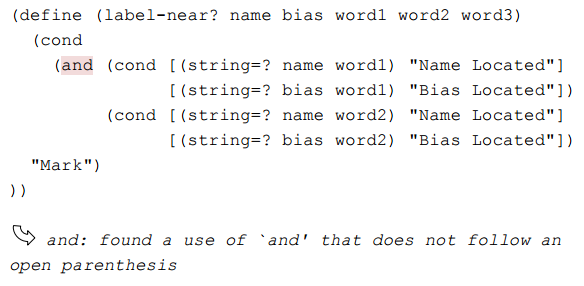
\includegraphics[keepaspectratio, width=0.5\textwidth]{MEE_example.png}
  \caption{Example of an ineffective error message in Racket}
  \label{fig:racketerrormessage}
\end{figure}

\todo[inline, color=orange]{simplify error message from figure 1, turn into verbatim}

Marceau, Fisler, and Krishnamurthi grouped messages into nine most common error categories in their results from the study.
Through their data collection at the end of the study, they found the percentage of occurrence of each error type from each lab as indicated by the \textit{\%error} and the percentage of students that responded poorly to the error message indicated as \textit{\%bad} as seen in figure 2.
\textit{\#bad} shows the level of likelihood of recurrence of the respective error message.
The values of interest are the \textit{\#bad} values enclosed in a box and the highest \textit{\%bad} values, as seen in figure \ref{fig:drracketstudy}). 

The data the authors gathered helped identify errors students found challenging.
The authors found that students have difficulties with certain errors at different points in the course, as expected since curricular aspects of the labs affect error patterns.
Many of the errors students struggled with were consistent with the course, such as difficulties with syntax errors in the first lab since students are still beginning to learn the language syntax.
However, the data is not entirely a representation of students' conceptual difficulties with the course, as Marceau et al. found.
The error messages a student receives, according to Marceau et al, ``is often not a direct indicator of the underlying error.''~\cite{Marceau:2011:MEE:1953163.1953308}
For example, in lab number six, numerous \texttt{unbound-id} errors  or unbound identifiers occurred, which is when the compiler finds a variable that was not defined.
However, the authors found that the actual problem students had was improperly using field reference operators and the actual errors they should have received was not given.
This suggests that there are some issues in the effectiveness of the error messages.

\begin{figure*}
  \centering
  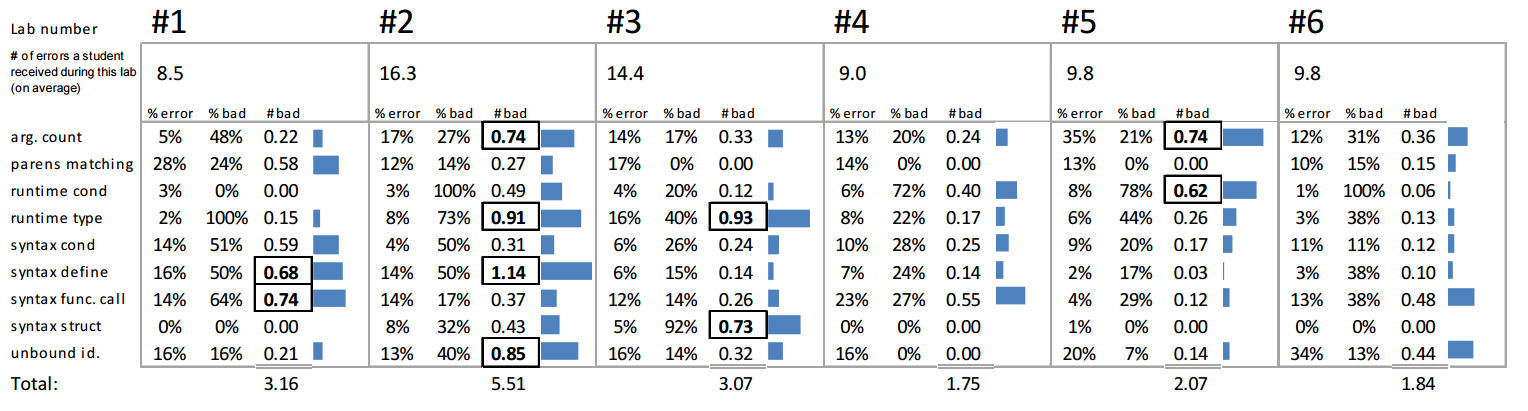
\includegraphics[keepaspectratio, width=\textwidth]{MEE_Data.png}
  \caption{Results from DrRacket study}
  \label{fig:drracketstudy}
\end{figure*}

\subsection{Analysis of compiler messages in C++}\label{subsec:compiler analysis}

\todo[inline, color=red]{still need to heavily edit section}

Compiler error messages are often cryptic and difficult to understand for many programmers, especially for students who are new to programming.
Unfortunately, as Traver notes, ``most related disciplines, including compiler technology, have not paid much attention to this important aspect that affects programmers significantly, apparently because it is felt that programmers should adapt to compilers.'' ~\cite{Traver:2010}
Not a lot of research has been conducted on compiler error message design.
In the first semester of 2002-2003, Traver conducted a case study on students' work with compiler error messages in C++ in an introductory computer science course.
The motivation of this study is to gain insight on what students are struggling with in the course and to help the professor's personal struggles with these error messages.
Traver gathered data from the students' interactions with C++ throughout the semester and wrote up analyses of the error messages received in 5 separate parts.
\begin{itemize}
	\item \textit{The error message} received from the compiler
	\item \textit{The source code} that caused the original error
	\item \textit{The diagnostic} of why the error occurred
	\item \textit{An alternate error message} that may help lead more directly to the true diagnosis of the issue.
	\item \textit{A comment} about why the error message is not helpful
\end{itemize}

Below is an example of an error message in C++ analyzed in the study along with the source code ~\cite{Traver:2010} (in the interest of space, I have not included the other parts of the analysis):

\begin{verbatim}
Source Code:

class SavingAccount 
friend ostream & operator<<
ostream &os, const SavingAccount &sA);
};
\end{verbatim}

\begin{verbatim}
Error Message:

ANSI C++ forbids declaration 
'ostream' with no type 'ostream'
is neither function nor method; 
cannot be declared friend
parse error before '&'
\end{verbatim}

\todo[inline, color=orange]{find a better code snippet}

In this case, the user forgot to include a header file (iostream.h), so the compiler does not know what iostream is.
The error message however, did not suggest to include a header, a simple fix, where the original error message could easily confuse novice programmers.
The author of the study noted that this type of error message should ``convey a clear message that the programmer can quickly understand and that is useful for fixing the error'', but the error message given to the user would not accomplish this for students who are still new to programming~\cite{Traver:2010}.

Traver found from the study, that there is an apparent lack of thought put into the usability of compiler error messages and that many students, especially those new to programming, will have a hard time understanding these errors.
There was no quantitative data gathered on these error messages, but rather just a general observation of how students struggled working with the compiler error messages.
Traver noted that ``better [error messages] are possible'' and was able to provide alternative error messages for each of the ones analyzed ~\cite{Traver:2010}.
So, better error message design is possible, such that more efforts and time are put into compiler error message research. 

\section{Methodologies}\label{sec:methodologies}
In this section, we will be discussing three methodologies and tools meant to attempt to improve the usability of error messages or suggest improvements for error message design based on the analyses discussed in section 3.
The first methodology we discuss is a set of recommendations for improving the usability of error messages in IDEs, specifically in DrRacket.
The second approach discusses improving compiler error messages through a set of principles meant to increase usability of the messages.
For the third approach, we will discuss an attempt on enhancing syntax error messages in Java and the how well these syntax error messages improve over the original. 

\subsection{Recommendations for error messages in IDEs}\label{subsec:error message rubric}
After Marceau et al. analyzed their data from the case study (as detailed in section \ref{subsec:racket analysis}), they found that students struggled to respond to error messages.
Through their research, they were able to develop a list of proposed methods of improving error messages, specifically for DrRacket, ``but  should apply just as well in any other programming language used for teaching, including those with
graphical syntaxes.''~\cite{Marceau:2011:MYL:2048237.2048241}
They also wanted to maintain two integral principles in error message design for their proposals:

\begin{itemize}
	\item Error messages should not propose solutions as these solutions can lead students down the wrong path and can not cover every scenario a student may encounter.
	\item Error messages should not prompt students toward incorrect edits. Source highlighting can cause issues and when not correctly implemented can cause more errors.
\end{itemize}

The first recommendation is simplifying vocabulary used in error messages.
The authors found that while DrRacket is ``accurate and consistent in its use of technical vocabulary'', but ``some of its terms are overly precise relative to terms that students already know.~\cite{Marceau:2011:MYL:2048237.2048241}''
For example, the term \texttt{identifier} is used in DrRacket error messages. However, the term \texttt{variable} is a term students are more likely to be familiar with~\cite{Marceau:2011:MYL:2048237.2048241}.
However, they also argue that non-simplified vocabulary is appropriate for an introductory computer science course.
Rather, simplified vocabulary would be better suited at entry-level teachpacks in DrRacket, and the higher teachpacks later in the course would help students become familiar with the vocabulary.

Marceau et al. also wanted error messages to be explicit about inconsistencies, specifically with function or constructor usage.
They found that DrRacket highlights the source expression where the variable or constructor is called, but not the definition.
The highlighting suggest edits should be made in the expression, but the error can also occur within the definition of the variable or constructor, which does not get highlighted when an error like this occurs.
While an IDE may not be able to identify whether a definition or its usage is the issue, it should not steer students in the wrong direction.
Inconsistencies can occur in many other facets of a language, such as syntax errors, but an IDE should not steer students down the wrong path~\cite{Marceau:2011:MYL:2048237.2048241}.

The authors go on to propose error messages should highlight every reference and its corresponding code with a distinct color in order to help students match message terms to code fragments.
They believe this should help resolve ambiguity about highlighting and ambiguous references (an example of an ambiguous reference is highlighted in blue in figure 3).
Figure 3 shows an example of a color coded error message from ~\cite{Marceau:2011:MYL:2048237.2048241}.
The red highlights the definition, the green highlights the clause, and the blue highlights the reference.

\begin{figure}
  \centering
  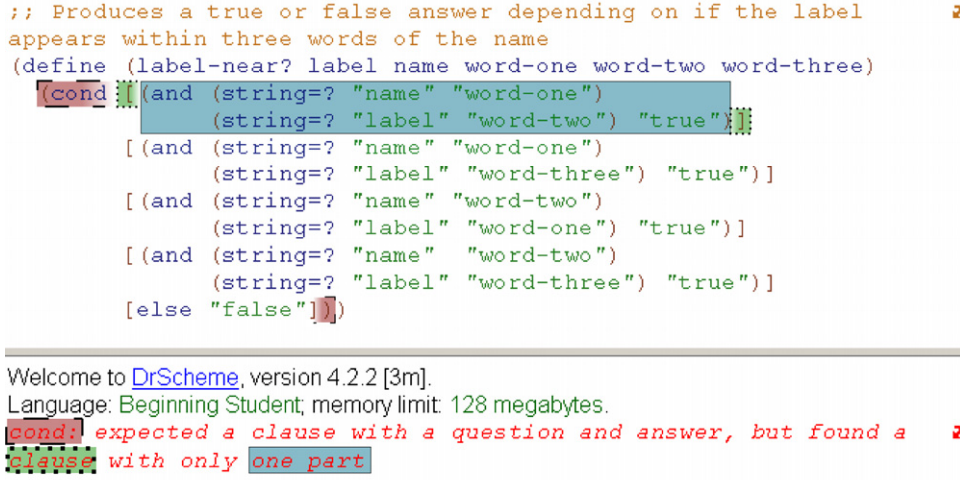
\includegraphics[keepaspectratio, width=0.5\textwidth]{DrRacketColorCodedMessage.png}
  \caption{Example of color coded message}
  \label{fig:colorcodedmessage}
\end{figure}

The last three recommendations are design suggestions for introductory courses that uses DrRacket to help students with error messages, so in the interest of space I will not be covering them.
These recommendations have not yet been implemented, but the authors hope to test them in the future~\cite{Marceau:2011:MYL:2048237.2048241}. 


%\subsection{Principles of compiler error design}\label{subsec:compiler error design}
%\todo[inline, color=red]{TODO}

\subsection{Syntax error message enhancement and results}\label{subsec:syntax enhancement}

Language syntax is often one of the first difficulties a student experiences when learning programming.~\cite{Denny:2011:USB:1999747.1999807}
Because of this, introductory students may see many syntax errors while learning the syntax of a language.
Denny et al. found that `` syntax errors can be a significant barrier to student success'' and thus propose to improve the existing error messages that deal with syntactical issues in a Java-based development environment for introductory programmers~\cite{Denny:2014:ESE:2591708.2591748}.

Denny et al. decided to implement the enhanced error message system through CodeWrite, a web-based tool for students to complete various Java exercises.
The code is entered directly in the browser and the students must write the body of a method, the header of the method is always provided.
In order to create the enhanced feedback, the authors began by examining student submissions in CodeWrite and found the errors that had ambiguous compiler error messages. 
They achieved this by performing an analysis of the code and use regular expressions to match commonly occurring patterns of code that caused errors and  extracting the line containing the error.
They then categorized the error messages according to error type by building a program called a recognizer that would parse source code and raw compiler error messages.
Once the original error is extracted, they then highlight the line and insert their enhanced error message.
The enhanced error messages contain the line number of the offending line of code and a detailed explanation of the error.
They also show an example of incorrect code and correct code of the corresponding syntax error with an explanation.
Figure 4 shows an example of an enhanced error message from the following code:~\cite{Denny:2014:ESE:2591708.2591748}

\begin{verbatim}
if (score < 0) || (score > 100)
Syntax error on token "||", if expected
\end{verbatim}

This statement is syntactically incorrect because the \texttt{if} statement is missing surrounding parenthesis. A syntactically correct statement would look like this:

\begin{verbatim}
if ((score < 0) || score > 100))
\end{verbatim}

\begin{figure*}
  \centering
  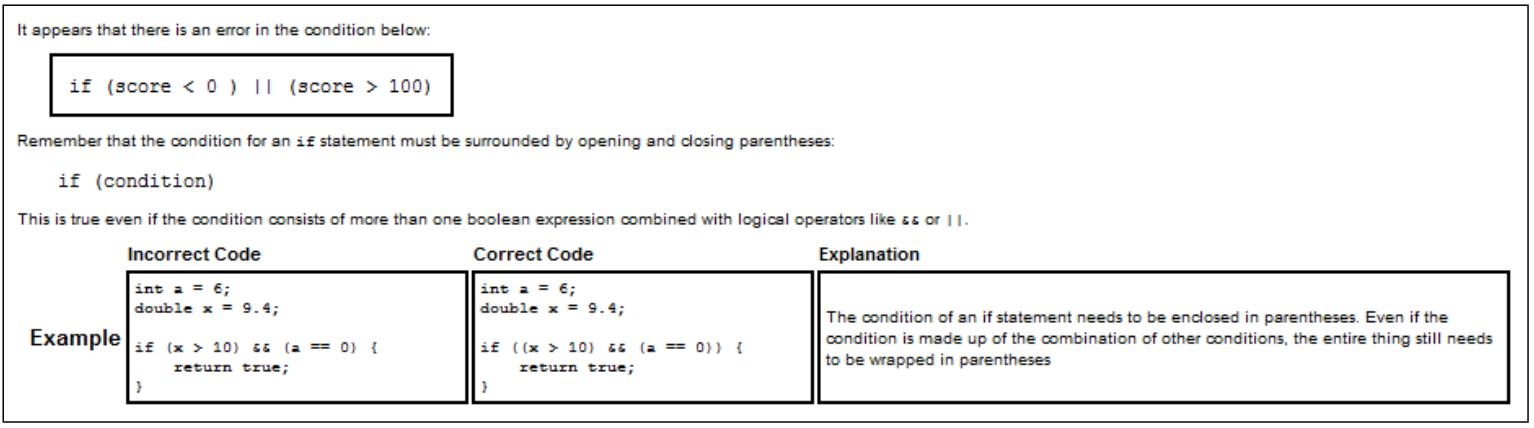
\includegraphics[keepaspectratio, width=\textwidth]{ESE_example.png}
  \caption{Example of an enhanced syntax error}
  \label{fig:drracketstudy}
\end{figure*}

The authors were interested in helping students improve their debugging skills, and were particularily interested in those who consistently submitted non-compiling code~\cite{Denny:2014:ESE:2591708.2591748}.
After creating these enhanced error messages, the authors wanted to examine whether they had an impact on:
\begin{itemize}
	\item The number of non-compiling submissions made while attempting an exercise
	\item The total number of non-compiler submissions
	\item The number of attempts needed to resolve most common kinds of errors
\end{itemize}

Denny et al had students in a summer course randomly put in a control group that received the original error message or the intervention that received their new error messages and submit their code in CodeWrite where the authors could be able to compare the submissions of the same exercise of each group.
Unfortunately, after testing whether their enhanced error messages had an impact on the above items, they found that their new feedback had no significant differences between the groups.

Denny et al found numerous possibilities for why their enhanced feedback system was not effective on helping introductory students improve their debugging skills.
They believed that the errors could have been simple enough to solve without needing to look at the messages.
Another possibility was that students did not put more attention into the additional information of the messages.
The authors hope to apply additional research into their enhanced errors to further find out why they were not any more helpful than the original messages~\cite{Denny:2014:ESE:2591708.2591748}.


\section{Conclusion}\label{sec:concl}

In this paper, we discussed compiler and runtime errors as well as dynamic and statically typed languages and how that affects error message handling.
We used that information to discuss studies done on error messages in DrRacket and C++ compiler error messages and how well introductory students can use them for debugging.
The research from DrRacket analysis concluded that students have difficulties with understanding error messages on unfamiliar concepts, but some errors in DrRacket incorrectly report the problem to the students and thus there is room for improvement.
The analysis on error messages from the compiler deduced that these messages are difficult to understand from an HCI perspective.
These are just two studies I analyzed in this paper, there are several others I looked over that discuss the quality of error messages for introductory students.

There is research being done on attempting to improve or suggest the improvement for the usability of error messages.
We discussed a set of recommendations on designing error messages which is geared toward assisting introductory students with debugging.
We also discussed a system of enhanced error messages for syntactical issues and that it was ineffective at helping students debug more than the original error messages.

\section{Future work}\label{sec:ftrwrk}

With the larger interest in the field of computer science and the growth in HCI studies, error message research, specifically for introductory programmers, has grown.
Marceau et al created a series of recommendations that they have implemented in HTDP teachpacks for DrRacket, which requires further research to find the effectiveness this has for introductory students.~\cite{htdp-teachpacks}.
Also, while Denny et al enhanced syntax error messages was ineffective, they hope to figure out why and improve upon them in the future through further research and interviews.
While it is crucial to retain an error message's educational standpoint, it is also important to ease new students into learning a programming language.
So, making sure the messages are user-friendly, such as familiar vocabulary or showing hints, is imperative to giving useful feedback for introductory students.


% The following two commands are all you need in the
% initial runs of your .tex file to
% produce the bibliography for the citations in your paper.
\bibliographystyle{acm}
% sample_paper.bib is the name of the BibTex file containing the
% bibliography entries. Note that you *don't* include the .bib ending here.
\bibliography{Usability_of_Error_Messages_for_Novice_Programmers}  

%\todo[inline, color=blue]{Citing sources for references}
%~\cite{Denny:2014:ESE:2591708.2591748}
%~\cite{Hartmann:2010:OPS:1753326.1753478}
%~\cite{Isa:1983:MOE:800045.801583}
%~\cite{Kummerfeld:2003:NBF:858403.858416}
%~\cite{Marceau:2011:MEE:1953163.1953308}
%~\cite{Marceau:2011:MYL:2048237.2048241}
%~\cite{Murphy:2008:BTD:1352135.1352193}
%~\cite{Traver:2010}
%~\cite{Denny:2011:USB:1999747.1999807}
% You must have a proper ".bib" file
%  and remember to run:
% latex bibtex latex latex
% to resolve all references

\end{document}
